\title{Assignment 4 -- CSC 225}
\author{
	Andrew \bf{Hobden} \\
	Student Number: \bf{V00788452}\\
	Instructor: Venkatesh Srinivasan
}
\date{\today}

\documentclass[12pt]{article}
\usepackage{mathtools}
\usepackage{amssymb}
\usepackage{algpseudocode}
\usepackage{algorithm}

\begin{document}
\maketitle

\section{BST Construction}
Insert items with the following keys (in the given order) into an initially empty binary search tree: 
62, 78, 44, 50, 48, 88, 17, 54
Draw the tree after each insertion. Is this an AVL tree?

\paragraph{Answer}
Yes, it's an AVL Tree. It is both a tree and satisfies the height balance property. Observe the labelled heights on the final step of the diagram. Since $3-2=1$ the height balance property is satisfied.
\clearpage
\begin{center}
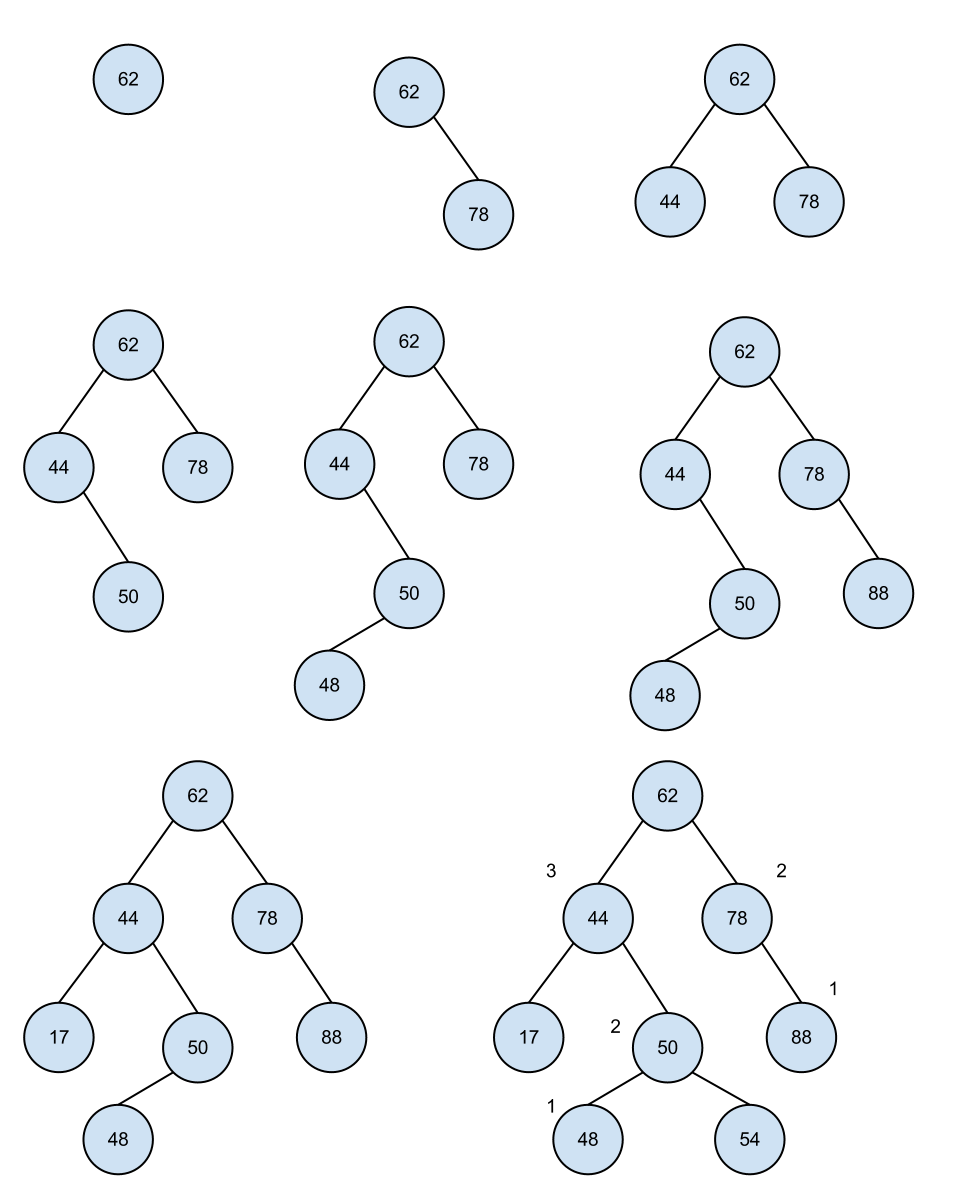
\includegraphics[width=0.9\textwidth]{figures/bst.png}
\end{center}

\section{AVL Insertion}
Draw the AVL tree resulting from the insertion of an item with key 52 into the tree you get from solving Problem 1.
\begin{center}
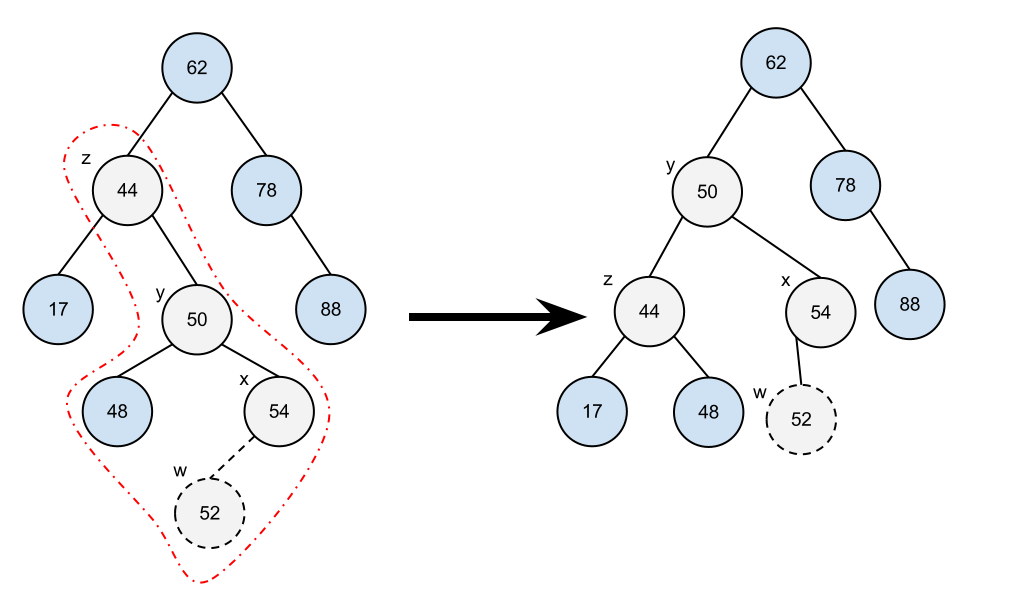
\includegraphics[width=0.9\textwidth]{figures/bst-insert.png}
\end{center}
Since $y(50)$ is $B$, $z(44)$ is $A$, and $x(54)$ is $C$, we'll arrange $y$ to be the new 'root'.
\section{AVL Removal}
Draw the AVL tree resulting from the removal of the item with key 62 from the tree you get from solving Problem  1.
We'll assume we're using the {\bf in-order predecessor} of the deleted node as the new root.
\paragraph{Reasoning}
This has an advantage (In this case) over using the in-order successor in that no restructure is needed. Choosing the other method is equally as valid and would possibly require tri-node restructure(s).
If we were to use in-order successor, we would traverse the tree from the replacement to the root, performing restructures wherever the height balance property is unsatisfied.

\paragraph{In-order Predecessor Based Removal}
\begin{center}
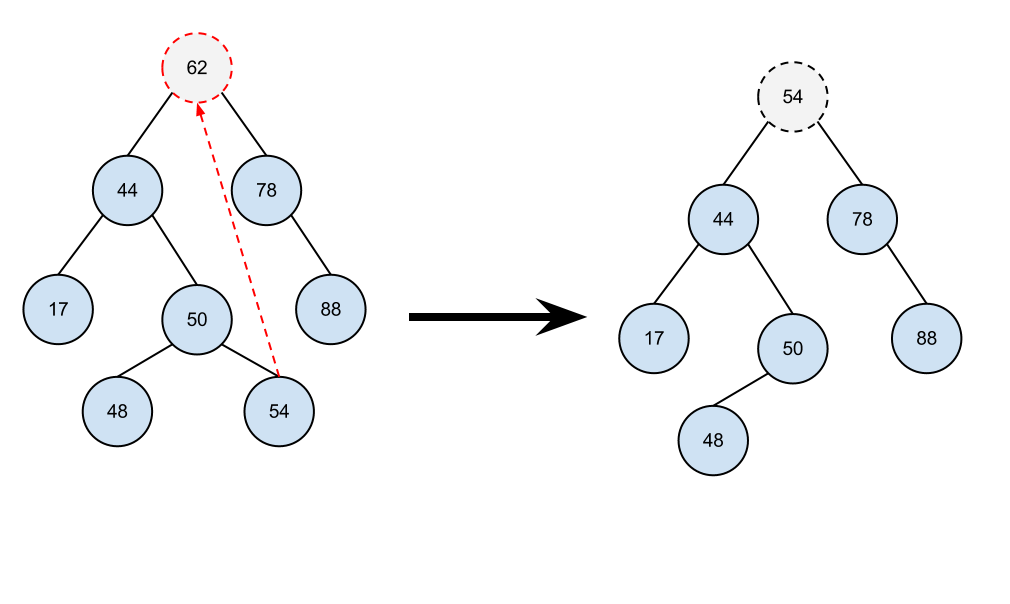
\includegraphics[width=0.9\textwidth]{figures/bst-remove.png}
\end{center}

\section{Restructure Upper Bounds}
Prove that at most one tri-node restructure operation is needed to restore balance after any insertion in an AVL tree.
%TODO Thoughts -- This sounds like an induction type proof. Any AVL must satisfy such and such, so adding one vertex means that to restore balance you only need to restore to such and such sub tree.
\paragraph{State Before Insertion}
Since this is an AVL tree, prior to insertion the height balance property is satisfied. This means that the difference in height between the two child nodes of any given node is either $0$ or $1$.
\subsection{Difference of 0} Given nodes with a height difference of 0, any insertion would (in worst case) give the nodes a height difference of 1. Since this still satisfies the height balance property {\bf this already holds.}
\subsection{Difference of 1} Given nodes with a height difference of 1, an insertion could potentially cause a restructure because of the height difference becoming $2$.
Since every other node in the tree already satisfied in regards to the height balance property (Since it is an AVL tree), if we can prove that a restructure will restore the node to a height difference of at most 1, then this holds.
We'll consider the 4 cases of restructure operations, they will 'pass' if they restore the height difference to either 0 or 1, from two.
\paragraph{Left Left Case}
\begin{center}
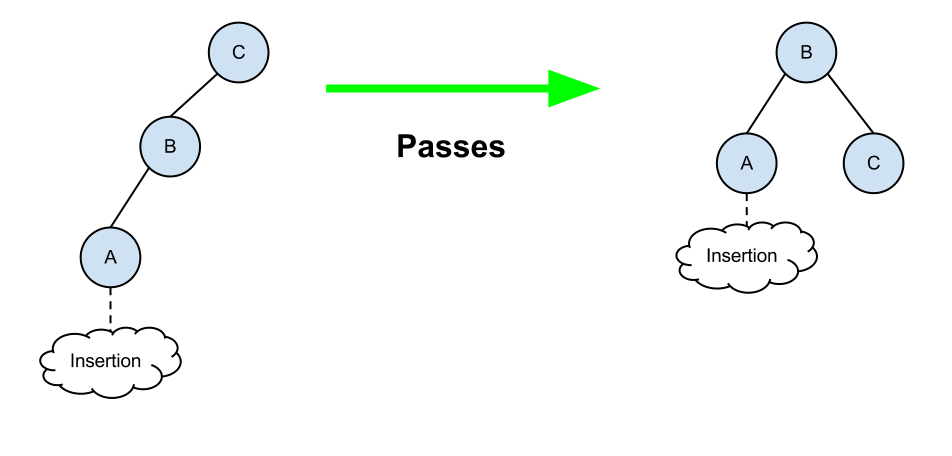
\includegraphics[width=0.8\textwidth]{figures/avl-case1.png}
\end{center}
\paragraph{Left Right Case}
\begin{center}
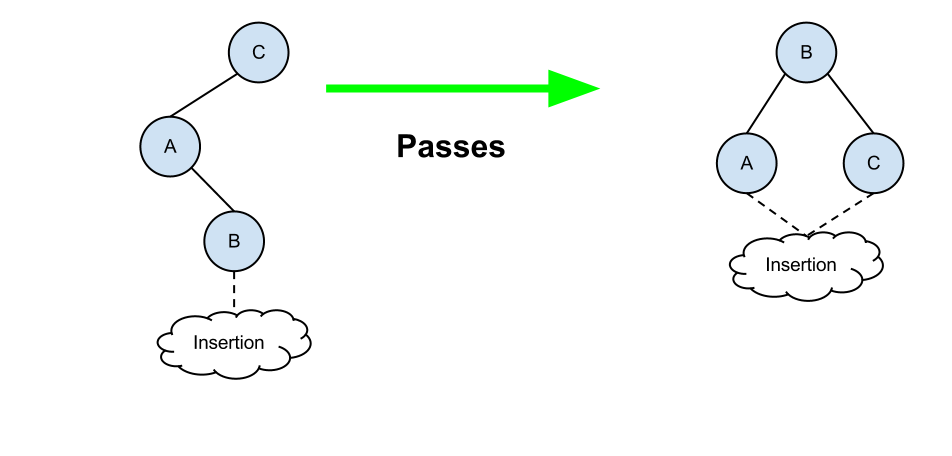
\includegraphics[width=0.8\textwidth]{figures/avl-case2.png}
\end{center}
\paragraph{Right Right Case}
\begin{center}
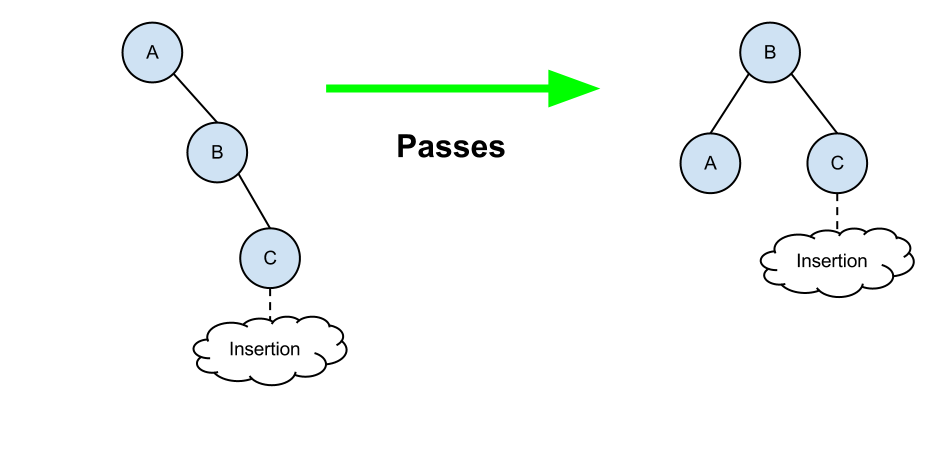
\includegraphics[width=0.8\textwidth]{figures/avl-case3.png}
\end{center}
\paragraph{Right Left Case}
\begin{center}
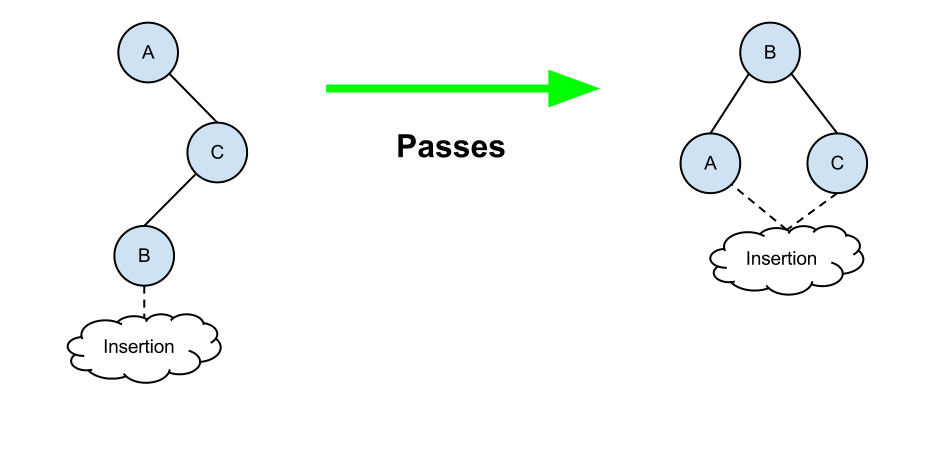
\includegraphics[width=0.8\textwidth]{figures/avl-case4.png}
\end{center}
\paragraph{Result}
Since all four possible cases provided a resultant (sub)tree of height difference 0 or 1, {/bf this holds.} Therefore this is proven.

\section{Depth First Search on a Graph}
Let G be a graph on 8 vertices labeled 1 through 8 and let the adjacent vertices of each vertex be given by the table below:
\begin{center}
\begin{tabular}{ c | c }
	Vertex & Adjacent Vertices \\
	1 & (2,3,4) \\
	2 & (1,3,4) \\
	3 & (1,2,4) \\
	4 & (1,2,3,6) \\
	5 & (6,7,8) \\
	6 & (4,5,7) \\
	7 & (5,6,8) \\
	8 & (5,7) \\
\end{tabular}
\end{center}
Assume that, in the traversal of G, the adjacent vertices of a given vertex are visited in the same order as they are listed in the above table.
\subsection{Depth First Search}
Order the vertices as they are visited in a DFS traversal starting at vertex 1.\\
%TODO Thoughts -- This should be easy.
Starting at vertex 1:
$1 \rightarrow 2 \rightarrow 3 \rightarrow 4 \rightarrow 6 \rightarrow 5 \rightarrow 7 \rightarrow 8 \rightarrow Done$
\subsection{Breadth First Search}
Order the vertices as they are visited in a BFS traversal starting at vertex 1.\\
%TODO Thoughts -- This should be easy.
Starting at vertex 1:
$1 \rightarrow 2 \rightarrow 3 \rightarrow 4 \rightarrow 6 \rightarrow 5 \rightarrow 7 \rightarrow 8 \rightarrow Done$
\section{Connectivity and Removal}
Prove that every connected graph has a vertex whose removal will not disconnect the graph. Describe an algorithm that finds such a vertex.
\paragraph{Assumptions}
A graph is connected if every pair of vertices is connected. This means there is a path from  $u$ to $v$ for every $u,v$. Cycles are allowed. The graph is {\bf undirected}.
\paragraph{Already Satisfied Cases}
The one and two vertex cases are already satisfied since if we remove a vertex from them, there are no more edges (and only at most one vertex, which would be connected.)
\subsection{Proof}
Since we know our graph is connected it must have a {\bf spanning tree}, which we will consider. Since any spanning tree with more then 1 vertex (noting that ours has at least 3, from the above) must have a least 2 leaves, we can safely say the original graph must have a least 1 vertex which can be removed without breaking connectivity.
\subsection{Pseudocode}
Our algorithm will perform the following steps:
\begin{itemize}
	\item Perform a BFS
	\item If it detects a single edged vertex, return it
	\item Otherwise, return the last item found in the BFS
\end{itemize}
\paragraph{Explanation}
If we find a single vertex, we can (obviously) remove it and maintain connectivity, since the vertex is not connecting anything but it's vertex to the rest of the graph. \\
If we don't find one, that means our graph has a cycle (Since there are no 'leaves'). Since we have performed a BFS, when we get to the last node found we already know that we have traversed all nodes in the graph other then the current node, therefore the rest of the graph must be connected and the last node can be safely removed without disconnection.
\begin{algorithm}
\begin{algorithmic}[1]
	\Function{nonCutVertexFind}{$Graph$, $start$}
		\State queue $\gets$ new Queue
		\State queue.enqueue($start$)
		\State mark $start$
		\While{Q is not empty}
			\State current $\gets$ queue.dequeue()
			\If{current.numOfEdges is 1}
				\State \Return current
			\EndIf
			\For{each edge in current.adjacentEdges}
				\If{edge is not marked}
					\State queue.enqueue(edge)
				\EndIf
			\EndFor
			\State lastVertex $\gets$ current
			\Comment Store the last vertex visited
		\EndWhile
		\State \Return lastVertex
		\Comment Return the last vertex found by the BFS
	\EndFunction
\end{algorithmic}
\end{algorithm}
%TODO Thoughts -- One and Two vertex case are solved because we're removing a vertex, not an edge. Furthermore the definition is: A graph is connected if every pair of vertices is connected.
\end{document}